\documentclass[aspectratio=169,10pt]{beamer}
\usetheme{metropolis}
\usepackage{amsmath,amssymb,bm}
\usepackage{siunitx}
\usepackage{booktabs}
\usepackage{tikz}
\usetikzlibrary{arrows.meta,calc,positioning,patterns}
\usepackage{pgfplots}
\pgfplotsset{compat=1.17}
\sisetup{per-mode=symbol,detect-all}
\DeclareSIUnit{\MParm}{MPa\,\ensuremath{\sqrt{\text{m}}}}
\metroset{numbering=fraction,progressbar=frametitle,block=fill}
\tikzset{capt/.style={text width=5.2cm,align=center}}
\hypersetup{colorlinks=true,urlcolor=blue!60!black,linkcolor=.}
% ITU logo on every frame (top-right): white on the dark title bar, navy on the title page.
\addtobeamertemplate{frametitle}{}{%
  \begin{tikzpicture}[remember picture,overlay]
    \node[anchor=north east,yshift=-1.5pt,xshift=-6pt] at (current page.north east) {
\includegraphics[height=0.7cm]{logos/itu_logo_beyaz.pdf}};
  \end{tikzpicture}}
\titlegraphic{\hfill
\includegraphics[height=1.6cm]{logos/itu_logo_laci.pdf}}

\title{Lecture 3: Fracture Mechanics and Damage Tolerance}
\subtitle{UCK 364E Design of Machine Elements}
\author{Prof.\ Dr.\ Onur Tunçer}
\institute{Department of Aeronautical Engineering, Istanbul Technical University}
\date{Fall 2026}

\begin{document}
\maketitle

\begin{frame}{Today}
\begin{enumerate}
  \item Why the previous lecture is not enough
  \item Why ordinary stress analysis fails at a crack
  \item The stress intensity factor $K_{\mathrm I}=\beta\sigma\sqrt{\pi a}$
  \item Fracture toughness, constraint, and the strength--toughness trade
  \item Fatigue crack growth and the Paris law
  \item Residual strength and the critical crack
  \item The inspection interval --- where it all comes together
  \item Safe-life, fail-safe, damage tolerance
  \item Three worked examples
\end{enumerate}
\end{frame}

\section{Why the previous lecture is not enough}

\begin{frame}{Last time we predicted \emph{initiation}}
S--N for long lives, $\varepsilon$--N for notches. Both assume the material starts out sound and stop at the moment a crack appears.
\vspace{4pt}
\begin{itemize}
  \item \alert{Real structure contains flaws from the start} --- inclusions, scratches, burrs at drilled holes, corrosion pits, the torn edge of a punched rivet hole. Initiation may be absent entirely
  \item \alert{Initiation scatter is enormous} --- a factor of ten or more. Crack \emph{growth} is far more repeatable, so predictions built on it are more trustworthy
  \item \alert{A crack is survivable if you find it} --- the whole modern philosophy
\end{itemize}
\begin{alertblock}{The question changes}
Lecture 2: \emph{how long until a crack appears?}\\
Lecture 3: \emph{given that a crack exists, how long until it is dangerous --- and how often must I look?}
\end{alertblock}
\end{frame}

\section{Why stress analysis fails at a crack}

\begin{frame}{An ellipse flattened into a crack}
\begin{columns}[T]
\column{0.44\textwidth}
\[
K_t=1+2\frac{a}{b}=1+2\sqrt{\frac{a}{\rho}}
\]
\begin{itemize}\footnotesize
  \item Circular hole ($a=b$): the familiar $K_t=3$
  \item As $\rho\to0$: \alert{$K_t\to\infty$}
  \item Elasticity says the stress at a sharp crack tip is infinite \emph{whatever} the load
\end{itemize}
\vspace{2pt}
But cracked structures carry load, and identical cracks fail at the same stress. \alert{Something other than the peak stress controls fracture.}
\column{0.56\textwidth}
\centering
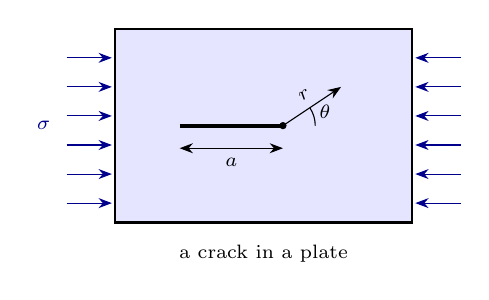
\begin{tikzpicture}[scale=0.82,>=Stealth,font=\scriptsize]
\begin{scope}
\fill[blue!10] (0,0) rectangle (4.6,3.0);
\draw[thick] (0,0) rectangle (4.6,3.0);
\draw[line width=1.4pt] (1.0,1.5) -- (2.6,1.5);
\fill (2.6,1.5) circle (1.6pt);
\draw[->] (2.6,1.5) -- (3.5,2.1) node[midway,above,sloped] {$r$};
\draw (3.1,1.5) arc (0:33:0.5); \node at (3.25,1.72) {$\theta$};
\foreach \y in {0.3,0.75,...,2.9} {\draw[->,blue!55!black] (-0.75,\y) -- (-0.05,\y); \draw[->,blue!55!black] (5.35,\y) -- (4.65,\y);}
\node[blue!55!black,anchor=east] at (-0.85,1.5) {$\sigma$};
\draw[<->] (1.0,1.15) -- (2.6,1.15) node[midway,below] {$a$};
\node[anchor=north] at (2.3,-0.2) {a crack in a plate};
\end{scope}
\end{tikzpicture}
\end{columns}
\end{frame}

\begin{frame}{Irwin's resolution: characterise the \emph{field}, not the peak}
\begin{columns}[T]
\column{0.54\textwidth}
Near the tip of a crack in a linear elastic body,
\[
\sigma_{ij}(r,\theta)=\frac{K}{\sqrt{2\pi r}}\,f_{ij}(\theta)+\dots
\]
\begin{itemize}\footnotesize
  \item The $r^{-1/2}$ singularity and the angular functions $f_{ij}(\theta)$ are \alert{the same for every crack in every body}
  \item All of the geometry and loading sits in the single scalar $K$
\end{itemize}
\column{0.46\textwidth}
\centering
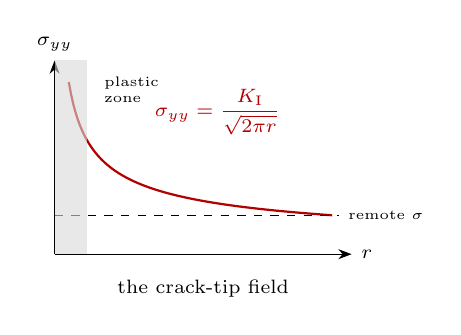
\begin{tikzpicture}[scale=0.82,>=Stealth,font=\scriptsize]
\begin{scope}
\draw[->] (0,0) -- (4.6,0) node[right] {$r$};
\draw[->] (0,0) -- (0,3.0) node[above] {$\sigma_{yy}$};
\draw[domain=0.22:4.3,samples=120,thick,red!70!black] plot (\x,{1.25/sqrt(\x)});
\draw[dashed] (0,0.6) -- (4.4,0.6) node[right,font=\tiny] {remote $\sigma$};
\node[red!70!black,anchor=west] at (1.4,2.2) {$\sigma_{yy}=\dfrac{K_{\mathrm I}}{\sqrt{2\pi r}}$};
\fill[gray!30,opacity=0.6] (0,0) rectangle (0.5,3.0);
\node[anchor=west,font=\tiny,align=left] at (0.62,2.55) {plastic\\ zone};
\node[anchor=north] at (2.3,-0.25) {the crack-tip field};
\end{scope}
\end{tikzpicture}
\end{columns}
\vspace{2pt}
\begin{block}{Linear elastic fracture mechanics, in one sentence}
Two different cracked components with the same $K$ have the same crack-tip conditions and behave the same way.
\end{block}
\scriptsize Three modes: I opening, II sliding, III tearing. Mode I dominates --- a crack under mixed loading turns normal to the maximum principal stress, converting itself into Mode I.
\end{frame}

\section{The stress intensity factor}

\begin{frame}{$K_{\mathrm I}=\beta\,\sigma\sqrt{\pi a}$}
\footnotesize
\begin{tabular}{@{}llp{6.8cm}@{}}
\toprule
Configuration & $\beta$ & Note \\
\midrule
Central crack $2a$, infinite plate & $1.00$ & the reference case \\
Edge crack $a$, semi-infinite plate & $1.12$ & the free edge relieves constraint \\
Two cracks at a hole, $a\gg R$ & $\approx1.0$ & $a$ measured from the hole centre \\
Short crack at a hole, $a\ll R$ & $\approx 3.4$ & the crack lies in the $K_t$ field of the hole \\
Embedded penny crack & $2/\pi=0.64$ & fully constrained \\
Surface semi-elliptical crack & $0.7$--$1.1$ & depends on $a/c$ and $a/t$ \\
Central crack, plate of width $W$ & $\sqrt{\sec(\pi a/W)}$ & finite-width correction \\
\bottomrule
\end{tabular}
\vspace{4pt}

\normalsize
\begin{alertblock}{Three things students get wrong}
\footnotesize
\textbf{1.} $K\neq K_t$. $K_t$ is dimensionless and describes a \emph{notch}; $K_{\mathrm I}$ is in \si{\MParm} and describes a \emph{crack}.\\
\textbf{2.} $\sigma$ is the stress that would exist \emph{without} the crack --- not a local stress.\\
\textbf{3.} $K\propto\sqrt{a}$: doubling the crack raises $K$ by only 41\%. That is why growth is slow at first and catastrophic at the end.
\end{alertblock}
\end{frame}

\begin{frame}{The plastic zone --- and when LEFM is allowed}
\[
r_p=\frac{1}{2\pi}\left(\frac{K_{\mathrm I}}{\sigma_y}\right)^{2}\ \text{(plane stress)},\qquad
r_p=\frac{1}{6\pi}\left(\frac{K_{\mathrm I}}{\sigma_y}\right)^{2}\ \text{(plane strain)}
\]
\begin{itemize}
  \item Infinite stress is impossible, so a small zone yields at the tip
  \item LEFM is valid only while that zone is small --- \alert{small-scale yielding}
  \item Rule of thumb: crack, ligament and thickness each $>2.5(K/\sigma_y)^2$
\end{itemize}
\begin{block}{When it is not valid}
Elastic--plastic methods: $J$-integral, CTOD, or an $R$-curve. \alert{Thin aluminium fuselage skin is usually in this regime} --- which is why residual strength there uses crack-tip opening angle, not a single toughness number.
\end{block}
\end{frame}

\section{Fracture toughness}

\begin{frame}{$K_{\mathrm I}=K_{\mathrm{Ic}}$ --- and why thickness matters}
\begin{columns}[T]
\column{0.52\textwidth}
$K_{\mathrm{Ic}}$ is the \alert{plane-strain} fracture toughness, measured to ASTM E399 on a specimen thick enough to guarantee plane strain:
\[
B,\;a,\;(W-a)\ \ge\ 2.5\left(\frac{K_{\mathrm{Ic}}}{\sigma_y}\right)^{2}
\]
\column{0.48\textwidth}
\textbf{Constraint}
\begin{itemize}\footnotesize
  \item \textbf{Thin}: free to contract through the thickness $\Rightarrow$ plane stress, big plastic zone, \emph{high} apparent $K_c$
  \item \textbf{Thick}: contraction prevented $\Rightarrow$ plane strain, small zone, toughness falls to its \emph{minimum} $K_{\mathrm{Ic}}$
  \item Beyond the transition thickness it stops falling
\end{itemize}
\end{columns}
\vspace{4pt}
\begin{alertblock}{}
Design with $K_{\mathrm{Ic}}$ unless you can justify the thin-section value by test.
\end{alertblock}
\end{frame}

\begin{frame}{Toughness and the critical crack}
\centering\footnotesize
\begin{tabular}{@{}lS[table-format=4]S[table-format=2.0]S[table-format=3.1]p{4.4cm}@{}}
\toprule
Material & {$\sigma_y$ (MPa)} & {$K_{\mathrm{Ic}}$} & {$a_c$ (mm)$^{*}$} & Comment \\
\midrule
2024-T3 sheet & 289 & 37 & 46.3 & damage tolerant; fuselage skin \\
7075-T6 & 462 & 24 & 19.5 & high strength, low toughness \\
7075-T73 & 400 & 31 & 32.5 & overaged: toughness bought with strength \\
7050-T7451 plate & 427 & 33 & 36.8 & thick fittings \\
Ti-6Al-4V (ann.) & 827 & 75 & 190.1 & excellent combination \\
4340 (1800 MPa) & 1517 & 50 & 84.5 & modest toughness \\
300M (1900 MPa) & 1600 & 65 & 142.8 & landing gear --- toughness is why \\
\bottomrule
\end{tabular}

\raggedright\vspace{3pt}
{\tiny $^{*}a_c$ for a central crack ($\beta=1$) at $\sigma=0.5\sigma_y$. $K_{\mathrm{Ic}}$ in \si{\MParm}. Classroom values only.}
\vspace{2pt}

\normalsize
\begin{alertblock}{The strength--toughness trade, quantified}
\footnotesize 7075-T6 is 60\% stronger than 2024-T3 --- and its critical crack is less than half as long. That is exactly why the \emph{lower} wing surface and the fuselage are 2024, and the \emph{upper} wing surface is 7075. Not ``which alloy is better'' but ``which failure mode governs here''.
\end{alertblock}
\end{frame}

\section{Fatigue crack growth}

\begin{frame}{The $\mathrm{d}a/\mathrm{d}N$ curve}
\centering
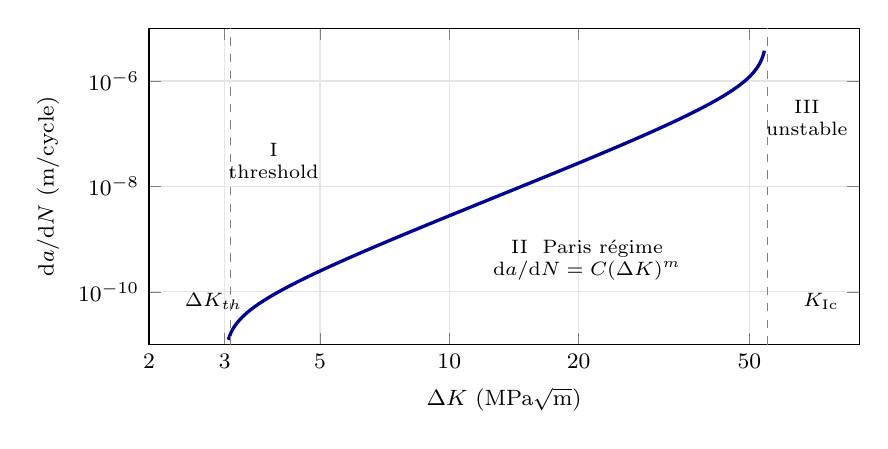
\begin{tikzpicture}
\begin{loglogaxis}[width=10.6cm,height=5.6cm,xlabel={$\Delta K$ (MPa$\sqrt{\text{m}}$)},ylabel={$\mathrm{d}a/\mathrm{d}N$ (m/cycle)},
 xmin=2,xmax=90,ymin=1e-11,ymax=1e-5,grid=both,grid style={gray!20},
 xtick={2,3,5,10,20,50},xticklabels={2,3,5,10,20,50},
 label style={font=\footnotesize},tick label style={font=\footnotesize}]
\addplot[very thick,blue!60!black,domain=3.06:54.2,samples=400]
  {3e-12*x^3*sqrt(1-3/x)/sqrt(1-x/55)};
\draw[gray,dashed] (axis cs:3.1,1e-11) -- (axis cs:3.1,1e-5);
\draw[gray,dashed] (axis cs:55,1e-11) -- (axis cs:55,1e-5);
\node[font=\scriptsize,anchor=south west] at (axis cs:2.3,3e-11) {$\Delta K_{th}$};
\node[font=\scriptsize,anchor=south east] at (axis cs:85,3e-11) {$K_{\mathrm{Ic}}$};
\node[font=\scriptsize,align=center] at (axis cs:3.9,3e-8) {I\\ threshold};
\node[font=\scriptsize,align=center,anchor=west] at (axis cs:12,4e-10) {II\ \ Paris r\'egime\\ $\mathrm{d}a/\mathrm{d}N=C(\Delta K)^m$};
\node[font=\scriptsize,align=center] at (axis cs:68,2e-7) {III\\ unstable};
\end{loglogaxis}
\end{tikzpicture}
\vspace{-2pt}
\begin{columns}[T]
\column{0.33\textwidth}\footnotesize
\textbf{I --- threshold}\\
below $\Delta K_{th}$ cracks do not propagate
\column{0.33\textwidth}\footnotesize
\textbf{II --- Paris}\\
straight on log--log; most of the life; where you calculate
\column{0.33\textwidth}\footnotesize
\textbf{III --- unstable}\\
$K_{\max}\to K_{\mathrm{Ic}}$, growth runs away
\end{columns}
\end{frame}

\begin{frame}{The Paris law and the life integral}
\[
\frac{\mathrm{d}a}{\mathrm{d}N}=C\,(\Delta K)^{m},\qquad m\approx2.5\text{--}4
\]
Because $\Delta K\propto\sqrt{a}$, the rate goes as $a^{m/2}$: at $m=4$, \alert{a crack ten times longer grows a hundred times faster}.
\[
N_f=\frac{2}{(m-2)\,C\,\beta^{m}\,\Delta\sigma^{m}\,\pi^{m/2}}
\left[\frac{1}{a_i^{(m-2)/2}}-\frac{1}{a_f^{(m-2)/2}}\right]
\]
\begin{itemize}
  \item \alert{Life is dominated by $a_i$.} Halving the initial flaw beats doubling the final one
  \item \alert{The final crack size barely matters} --- at $m=4$ you can often take $a_f\to\infty$
  \item \alert{Life scales as $\Delta\sigma^{-m}$} --- a 10\% stress reduction buys $\approx$46\% more life at $m=4$
\end{itemize}
\footnotesize In practice $\beta$ varies with $a$: integrate numerically, cycle by cycle, with the Lecture 2 spectrum. That is what NASGRO and AFGROW do.
\end{frame}

\begin{frame}{Mean stress, closure, retardation}
\begin{columns}[T]
\column{0.5\textwidth}
\textbf{$R$-dependence}
\begin{itemize}\footnotesize
  \item At higher mean stress the crack is open for more of the cycle and grows faster
  \item Forman and NASGRO equations add this explicitly
\end{itemize}
\textbf{Crack closure}
\begin{itemize}\footnotesize
  \item The plastic wake behind the tip props the crack open
  \item Part of the nominal $\Delta K$ does no damage; only $\Delta K_{\text{eff}}$ drives growth
\end{itemize}
\column{0.5\textwidth}
\textbf{Retardation}
\begin{itemize}\footnotesize
  \item One large overload makes an oversized plastic zone the crack must grow through
  \item Growth slows or stops for thousands of cycles
\end{itemize}
\begin{alertblock}{But it is ignored}
\footnotesize Retardation is real and sometimes worth tens of percent of life --- yet it is normally \alert{not credited} in certification: relying on it is non-conservative, and a high--low sequence can equally produce \emph{acceleration}.
\end{alertblock}
\end{columns}
\end{frame}

\section{Residual strength}

\begin{frame}{The residual strength diagram}
\centering
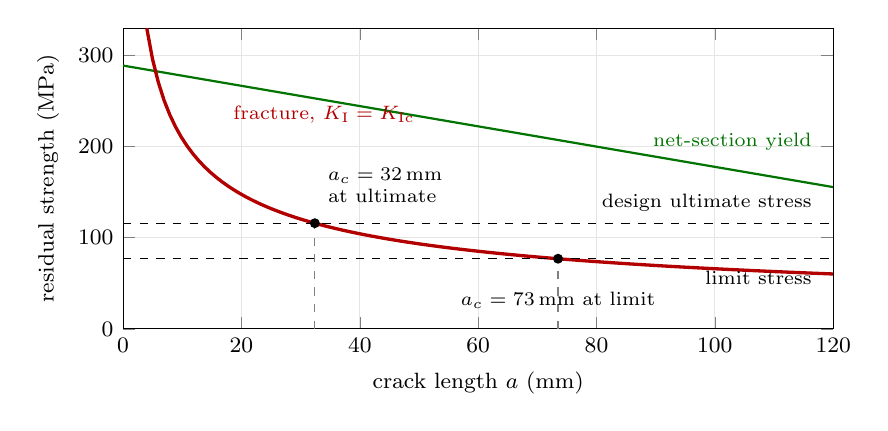
\begin{tikzpicture}
\begin{axis}[width=10.6cm,height=5.4cm,xlabel={crack length $a$ (mm)},ylabel={residual strength (MPa)},
 xmin=0,xmax=120,ymin=0,ymax=330,grid=both,grid style={gray!20},
 label style={font=\footnotesize},tick label style={font=\footnotesize}]
% net section yield line
\addplot[thick,green!45!black,domain=0:120,samples=2]{289*(1-x/260)};
% fracture line K=Kic
\addplot[very thick,red!70!black,domain=4:120,samples=120]{37/sqrt(3.1416*x/1000)};
% limit and ultimate
\draw[dashed,black] (axis cs:0,116) -- (axis cs:120,116);
\node[font=\scriptsize,anchor=south east] at (axis cs:118,118) {design ultimate stress};
\draw[dashed,black] (axis cs:0,77) -- (axis cs:120,77);
\node[font=\scriptsize,anchor=north east] at (axis cs:118,74) {limit stress};
% critical crack sizes, read off the fracture curve
\draw[gray,dashed] (axis cs:32.4,0) -- (axis cs:32.4,116);
\fill (axis cs:32.4,116) circle (1.8pt);
\node[font=\scriptsize,anchor=south west,align=left] at (axis cs:33,128) {$a_c=\SI{32}{mm}$\\ at ultimate};
\draw[gray,dashed] (axis cs:73.5,0) -- (axis cs:73.5,77);
\fill (axis cs:73.5,77) circle (1.8pt);
\node[font=\scriptsize,anchor=south,align=center] at (axis cs:73.5,12) {$a_c=\SI{73}{mm}$ at limit};
\node[font=\scriptsize,red!70!black,anchor=west] at (axis cs:17,235) {fracture, $K_{\mathrm I}=K_{\mathrm{Ic}}$};
\node[font=\scriptsize,green!45!black,anchor=east] at (axis cs:118,205) {net-section yield};
\end{axis}
\end{tikzpicture}
\vspace{-4pt}

\footnotesize 2024-T3, $K_{\mathrm{Ic}}=\SI{37}{\MParm}$, $\sigma_y=\SI{289}{MPa}$, central crack. Net-section yield governs when the crack is short; fracture governs when it is long.
\end{frame}

\begin{frame}{What ``critical'' means}
\begin{alertblock}{There is no single critical crack length}
There is a crack length that is critical \alert{at a stated stress}.
\end{alertblock}
\begin{itemize}
  \item CS-25.571 requires the \emph{cracked} structure to carry a specified residual-strength load --- commonly limit load, or a defined fraction, depending on the structural category and the inspection programme
  \item Choose the stress first, then read $a_c$ off the diagram
  \item From the figure: $a_c=\SI{32}{mm}$ at ultimate stress, $\SI{73}{mm}$ at limit stress --- \alert{same material, same panel}
\end{itemize}
\vspace{2pt}
\begin{block}{}
The critical crack size is a \emph{certification decision}, not a material property.
\end{block}
\end{frame}

\section{The inspection interval}

\begin{frame}{Six steps}
\begin{enumerate}\scriptsize
  \item Assume an initial flaw $a_0$ --- the largest that could escape manufacturing inspection; conventionally \SI{1.27}{mm} (0.05\,in) at a fastener hole
  \item Compute $a_c$ from the residual-strength requirement
  \item Integrate the growth law over the flight spectrum: the curve $a(N)$ from $a_0$ to $a_c$, total life $N_c$
  \item Determine the \alert{detectable} size $a_{\mathrm{det}}$ for the method you will specify
  \item The usable window runs from $a_{\mathrm{det}}$ to $a_c$: $N_{\mathrm{window}}$ flights
  \item Repeat interval $=N_{\mathrm{window}}/n$, with $n\ge2$ --- so at least two inspections occur while the crack is detectable but not yet critical
\end{enumerate}
\centering
\scalebox{0.86}{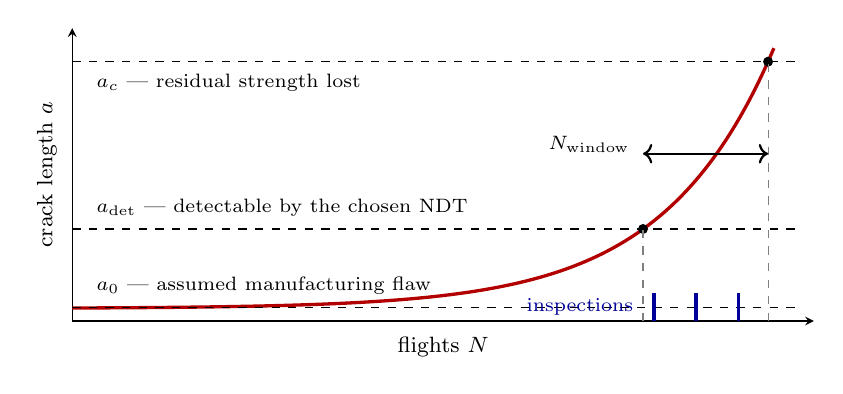
\begin{tikzpicture}
\begin{axis}[width=11.0cm,height=5.3cm,xlabel={flights $N$},ylabel={crack length $a$},
 xmin=0,xmax=1.02,ymin=0,ymax=1.05,xtick=\empty,ytick=\empty,axis lines=left,
 label style={font=\footnotesize}]
\addplot[very thick,red!70!black,domain=0:0.965,samples=240]{0.045+0.0016*exp(6.6*x)};
\draw[dashed] (axis cs:0,0.93) -- (axis cs:1.0,0.93);
\node[font=\scriptsize,anchor=north west] at (axis cs:0.02,0.92) {$a_c$ --- residual strength lost};
\draw[dashed] (axis cs:0,0.33) -- (axis cs:1.0,0.33);
\node[font=\scriptsize,anchor=south west] at (axis cs:0.02,0.34) {$a_{\mathrm{det}}$ --- detectable by the chosen NDT};
\draw[dashed] (axis cs:0,0.047) -- (axis cs:1.0,0.047);
\node[font=\scriptsize,anchor=south west] at (axis cs:0.02,0.06) {$a_0$ --- assumed manufacturing flaw};
% detectable / critical crossings
\fill (axis cs:0.785,0.33) circle (1.8pt);
\fill (axis cs:0.957,0.93) circle (1.8pt);
\draw[gray,dashed] (axis cs:0.785,0) -- (axis cs:0.785,0.33);
\draw[gray,dashed] (axis cs:0.957,0) -- (axis cs:0.957,0.93);
% window
\draw[<->,thick] (axis cs:0.785,0.60) -- (axis cs:0.957,0.60);
\node[font=\scriptsize,anchor=south east,align=right] at (axis cs:0.78,0.57) {$N_{\mathrm{window}}$};
% inspections
\draw[blue!60!black,very thick] (axis cs:0.800,0.0) -- (axis cs:0.800,0.10);
\draw[blue!60!black,very thick] (axis cs:0.858,0.0) -- (axis cs:0.858,0.10);
\draw[blue!60!black,very thick] (axis cs:0.916,0.0) -- (axis cs:0.916,0.10);
\node[font=\scriptsize,blue!60!black,anchor=east] at (axis cs:0.785,0.05) {inspections};
\end{axis}
\end{tikzpicture}}
\end{frame}

\begin{frame}{Detectability is a design parameter}
\centering\footnotesize
\begin{tabular}{@{}llp{6.8cm}@{}}
\toprule
Method & Typical $a_{\mathrm{det}}$ & Notes \\
\midrule
General visual, in service & \SIrange{25}{50}{mm} & unaided, walkaround distance \\
Detailed visual, close & \SIrange{5}{15}{mm} & clean surface, good light, unloaded \\
Dye penetrant & \SIrange{2}{5}{mm} & surface-breaking only, surface accessible \\
Eddy current, surface & \SIrange{1}{2}{mm} & finds cracks under rivet heads --- the Aloha method \\
Ultrasonic & \SIrange{1}{3}{mm} & subsurface; couplant, trained operator \\
X-ray & $\approx$2\% of thickness & poor for tight cracks normal to the beam \\
\bottomrule
\end{tabular}
\vspace{4pt}

\raggedright\normalsize
Formally detection is probabilistic: the \alert{probability of detection} curve, and the certification figure $a_{90/95}$ --- detected with 90\% probability at 95\% confidence.
\begin{alertblock}{The designer's lever is \emph{access}}
A crack that can only be found by removing an engine will be inspected rarely, the interval will be driven somewhere uneconomic --- or the part must be safe-life.
\end{alertblock}
\end{frame}

\begin{frame}{Why this is a design lecture, not a materials lecture}
Every item on the inspection-interval list is something \alert{you} control:
\begin{columns}[T]
\column{0.5\textwidth}
\begin{itemize}\footnotesize
  \item the initial flaw size --- hole quality, cold expansion, finish
  \item the stress range --- sizing, load path
  \item the critical crack size --- material, tear straps, crack stoppers
\end{itemize}
\column{0.5\textwidth}
\begin{itemize}\footnotesize
  \item the detectable size --- choice of method and, above all, \alert{access}
  \item the number of load paths
\end{itemize}
\end{columns}
\vspace{6pt}
\begin{alertblock}{}
A structure that is awkward to inspect is a \alert{design error}, not a maintenance problem.
\end{alertblock}
\end{frame}

\section{The three philosophies}

\begin{frame}{Safe-life, fail-safe, damage tolerance}
\footnotesize
\begin{description}
  \item[Safe-life.] Assumed crack-free; retired at (demonstrated life)/(scatter factor 3--5). No inspection credit. Landing-gear structure, engine discs, rotorcraft dynamic components. \alert{Weakness:} the scatter factor is a guess about variability --- the F-111 wing carry-through failure in 1969, at 100 flight hours from a forging defect, is the accident that discredited it for airframes.
  \item[Fail-safe.] Multiple load paths or crack-arrest features: after the complete failure of any one element the remainder carries a specified load long enough to be found. The dual-lug fitting from Lecture 1, and the tear straps that saved the Aloha aircraft.
  \item[Damage tolerance.] Cracks assumed present from the first flight. Growth calculated, residual strength demonstrated, inspection programme derived. \alert{The default for transport metallic structure}, and the inspection programme is part of the certified design.
\end{description}
\begin{alertblock}{WFD limits all of it}
\footnotesize Everything here assumes \emph{one} dominant crack in sound structure. Aloha 243 broke that assumption. Hence widespread fatigue damage in the regulations, and the \alert{Limit of Validity} --- a cycle count beyond which the aircraft may not fly without further substantiation, however good its inspection record.
\end{alertblock}
\end{frame}

\section{Worked examples}

\begin{frame}{Example 3.1 --- Critical crack in a fuselage skin}
2024-T3, hoop stress \SI{95}{MPa} at limit, $K_{\mathrm{Ic}}=\SI{37}{\MParm}$, central crack $\beta=1$
\[
a_c=\frac{1}{\pi}\left(\frac{K_{\mathrm{Ic}}}{\beta\sigma}\right)^{2}
=\frac{1}{\pi}\left(\frac{37}{95}\right)^{2}=\SI{48}{mm}
\]
\begin{itemize}
  \item So a through-crack of \SI{97}{mm} tip to tip is critical --- \alert{large and visible}, which is the point: 2024-T3 was chosen so the critical crack is big enough to find
  \item Same stress in 7075-T6 ($K_{\mathrm{Ic}}=\SI{24}{\MParm}$): $a_c=\SI{20}{mm}$, less than half
\end{itemize}
\begin{block}{Validity check}
$2.5(K/\sigma_y)^2=2.5(37/289)^2=\SI{41}{mm}\gg\SI{1.6}{mm}$ skin. The sheet is in \alert{plane stress}, so the real toughness is higher and this estimate is conservative --- but a thin skin properly needs an $R$-curve, not a single number.
\end{block}
\end{frame}

\begin{frame}{Example 3.2 --- Crack growth at a fastener hole}
7075-T6, $\Delta\sigma=\SI{80}{MPa}$, $R=0$, $a_i=\SI{1.27}{mm}$, $\beta=1.12$, $C=\SI{2.0e-11}{}$, $m=3.5$ (\si{m/cycle}, \si{\MParm}), $K_{\mathrm{Ic}}=\SI{24}{\MParm}$
\begin{align*}
a_f&=\frac{1}{\pi}\left(\frac{24}{1.12\times80}\right)^{2}=\SI{22.8}{mm}\\
(m-2)C\beta^m\Delta\sigma^m\pi^{m/2}&=1.5\times2.0{\times}10^{-11}\times1.487\times4.579{\times}10^{6}\times7.413=1.514{\times}10^{-3}\\
a_i^{-0.75}-a_f^{-0.75}&=148.6-17.0=131.6
\qquad\Rightarrow\qquad N_f=\frac{2\times131.6}{1.514{\times}10^{-3}}=\mathbf{1.74\times10^{5}}\ \text{cycles}
\end{align*}
\begin{alertblock}{Units --- the most common error in this subject}
\footnotesize $C$ is published in at least four unit systems; $m$ does not change between them, so a wrong $C$ is out by $10^3$ and still looks plausible on a log plot. \textbf{Sanity check:} aluminium at $\Delta K=\SI{10}{\MParm}$ should give a few $\times10^{-8}$\,m/cycle. Here $C(10)^{3.5}=\SI{6.3e-8}{m/cycle}$. Passes.
\end{alertblock}
\end{frame}

\begin{frame}{Example 3.3 --- Setting the interval}
Same lug, eddy current with $a_{90/95}=\SI{2}{mm}$, 1\,500 flights per year
\begin{align*}
N(1.27\to2\,\text{mm})&=\frac{2(148.6-105.7)}{1.514\times10^{-3}}=5.67\times10^{4}\ \text{flights}\\
N(1.27\to22.8\,\text{mm})&=1.74\times10^{5}\ \text{flights}\\
N_{\mathrm{window}}&=1.17\times10^{5}\ \text{flights}
\qquad\Rightarrow\qquad \text{interval}=\tfrac12 N_{\mathrm{window}}=5.9\times10^{4}\ (\approx39\ \text{years})
\end{align*}
\begin{alertblock}{Now change one thing}
The fitting is buried: general visual only, $a_{\mathrm{det}}=\SI{25}{mm}$. But $a_c=\SI{22.8}{mm}$ --- the crack is \alert{critical before it is detectable}. The window is negative and \alert{no inspection interval exists}.\\[2pt]
Options: lower the stress or raise the toughness ($a_c\uparrow$), provide access ($a_{\mathrm{det}}\downarrow$), add a second load path, or make it safe-life.
\end{alertblock}
\scriptsize This calculation costs ten minutes and decides whether a design is maintainable. Do it while the layout can still change.
\end{frame}

\section{For next time}

\begin{frame}{For next time}
\begin{itemize}
  \item Shigley \S\S5.12 and 6.5; Dowling Ch.\ 8 and 11 --- the best treatment at this level; Anderson Ch.\ 2--3
  \item Niu, \emph{Airframe Structural Design}, Ch.\ 15 (damage tolerance)
  \item \href{https://www.easa.europa.eu/en/document-library/easy-access-rules/online-publications/easy-access-rules-large-aeroplanes-cs-25}{CS-25.571 with AMC 25.571}, and FAA AC 25.571-1D for its worked treatment of inspection thresholds
  \item Self-study problems 1--6 in the notes (two are Python: a numerical Paris integrator with $\beta(a)$, and an interval calculation)
  \item Next: fatigue under combined loading --- multiaxial stress, rainflow counting and Miner's rule on a real flight spectrum
\end{itemize}
\end{frame}

\end{document}
